\documentclass[11pt,oneside]{article}
\usepackage[T1]{fontenc}
\usepackage[utf8]{inputenc}
%\DeclareUnicodeCharacter{00A0}{ }
\usepackage[adobe-utopia]{mathdesign}

\usepackage{amsmath}
\usepackage[francais]{babel}
\usepackage[dvips]{graphicx}
%\usepackage{here}
\usepackage{framed}
\usepackage[normalem]{ulem}
\usepackage{fancyhdr}
\usepackage{titlesec}
\usepackage{vmargin}

\usepackage{amsmath}
\usepackage{ifthen}
\usepackage{multirow}
\usepackage{multicol} % Portions de texte en colonnes

%\usepackage{xltxtra} % Logo XeLaTeX
%\usepackage{pst-solides3d}
\usepackage{color}
%\usepackage{colortbl}
\usepackage{titletoc} % Pour la mise en forme de la table des matières

%\usepackage[crop=off]{auto-pst-pdf}
%\usepackage{bclogo}


%\usepackage{longtable}
%\usepackage{flafter}%floatants après la référence
%\usepackage{pst-solides3d}
%\usepackage{pstricks}
%\usepackage{minitoc}
%\setcounter{minitocdepth}{4}
%\usepackage{draftcopy}% "Brouillon"
%\usepackage{floatflt}
%\usepackage{psfrag}
%\usepackage{listings} % Permet d'insérer du code de programmation
%\usepackage{lmodern}
%\usepackage[adobe-utopia,uppercase=upright,greeklowercase=upright]{mathdesign}
%\usepackage{minionpro}
%\usepackage{pifont}
%\usepackage{amssymb}
%\usepackage[francais]{varioref}

\setmarginsrb{1.5cm}{1cm}{1cm}{1.5cm}{1cm}{1cm}{1cm}{1cm}

\definecolor{gris25}{gray}{0.75}
\definecolor{bleu}{RGB}{18,33,98}
\definecolor{bleuf}{RGB}{42,94,171}
\definecolor{bleuc}{RGB}{231,239,247}
\definecolor{rougef}{RGB}{185,18,27}
\definecolor{rougec}{RGB}{255,230,231}
\definecolor{vertf}{RGB}{103,126,82}
\definecolor{vertc}{RGB}{220,255,191}
\definecolor{violetf}{RGB}{112,48,160}
\definecolor{violetc}{RGB}{230,224,236}
\definecolor{jaunec}{RGB}{220,255,191}

\usepackage{style/schemabloc}
%Si le boolen xp est vrai : compilation pour xabi
%Sinon compilation Damien
\newboolean{xp}
\setboolean{xp}{true}

\newboolean{prof}
\setboolean{prof}{true}

\def\xxtitre{\ifthenelse{\boolean{xp}}{
CI 2 -- SLCI : Étude du comportement des Systèmes Linéaires Continus Invariants}{
}}

\def\xxsoustitre{\ifthenelse{\boolean{xp}}{
Exercice de colle}{
}}


\def\xxauteur{\ifthenelse{\boolean{xp}}{
\noindent 2013 -- 2014 \\
Florestan \textsc{Mathurin}}{
}}


\def\xxpied{\ifthenelse{\boolean{xp}}{
CI 2 : SLCI\\
Exercice de colle \ifthenelse{\boolean{prof}}{P}{E}%
}{
}}

\usepackage[%
    pdftitle={SLCI - Systèmes du second ordre},
    pdfauthor={Xavier Pessoles},
    colorlinks=true,
    linkcolor=blue,
    citecolor=magenta]{hyperref}



\usepackage{pifont}
\sloppy
\hyphenpenalty 10000


\begin{document}






% \makeatletter \let\ps@plain\ps@empty \makeatother
%% DEBUT DU DOCUMENT
%% =================




%------------- En tetes et Pieds de Pages ------------


\pagestyle{fancy}
\ifthenelse{\boolean{xp}}{%
\renewcommand{\headrulewidth}{0pt}}{%
\renewcommand{\headrulewidth}{0.2pt}} %pour mettre le trait en haut
%\renewcommand{\headrulewidth}{0.2pt}

\fancyhead{}
\fancyhead[L]{%
\ifthenelse{\boolean{xp}}{%
\noindent\begin{minipage}[c]{2.6cm}%

\includegraphics[width=2cm]{png/logo_ptsi.png}%
\end{minipage}%
}{%
\footnotesize{\textit{\textsf{Lycée François Premier}}}
}}

\ifthenelse{\boolean{xp}}{%
\fancyhead[C]{\rule{12cm}{.5pt}}}{
}


\fancyhead[R]{%
\noindent\begin{minipage}[c]{3cm}
\begin{flushright}
\footnotesize{\textit{\textsf{Sciences Industrielles \\ de l'ingénieur}}}%
\end{flushright}
\end{minipage}
}


\ifthenelse{\boolean{xp}}{%
\fancyhead[C]{\rule{12cm}{.5pt}}}{
}

\renewcommand{\footrulewidth}{0.2pt}

\fancyfoot[C]{\footnotesize{\bfseries \thepage}}
\fancyfoot[L]{%
\begin{minipage}[c]{.2\linewidth}
\noindent\footnotesize{{\xxauteur}}
\end{minipage}
\ifthenelse{\boolean{xp}}{}{%
\begin{minipage}[c]{.15\linewidth}

\includegraphics[width=2cm]{png/logoCC.png}
\end{minipage}}
}


\fancyfoot[R]{\footnotesize{\xxpied}}



\begin{center}
 \Large\textsc{\xxtitre}
\end{center}

\begin{center}
 \large\textsc{\xxsoustitre}
\end{center}

%\vspace{.5cm}

\begin{center}
 \large\textsc{Robot préhenseur}
\end{center}

\begin{flushright}
\textit{D'après ressources Florestan Mathurin.}
\end{flushright}



Le support de l'étude est un préhenseur de pièces. Il permet à l'utilisateur de prendre des pièces pour les déplacer. L'application illustrée sur l'image ci-dessous est la prise de bouteilles plastiques sur un tapis roulant, afin de les trier pour faire du recyclage. 

\vspace{0.25cm}

\begin{center}
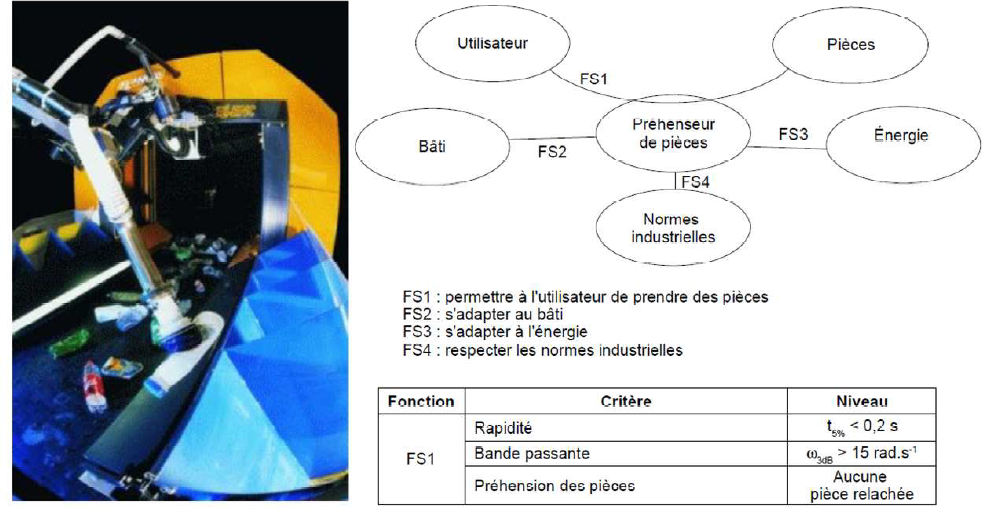
\includegraphics[width=.95\textwidth]{png/fig2}
\end{center}
%\begin{minipage}[c]{.3\linewidth}
%\begin{center}
%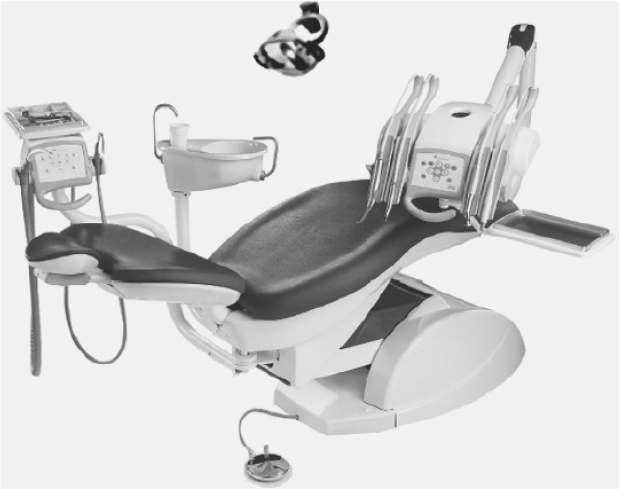
\includegraphics[width=.9\textwidth]{png/fig1}
%\end{center}
%\end{minipage}\hfill
%\begin{minipage}[c]{.65\linewidth}
%\begin{center}
%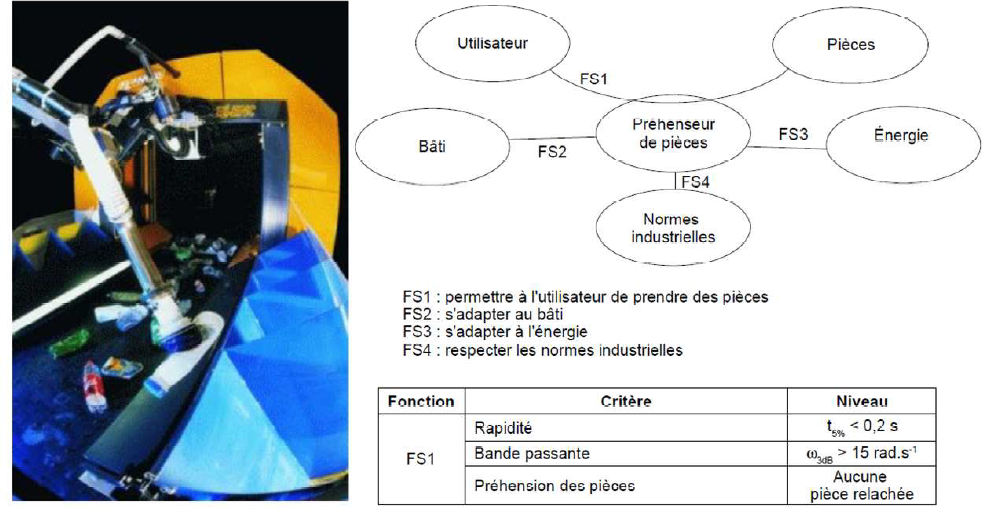
\includegraphics[width=.9\textwidth]{png/fig2}
%\end{center}
%\end{minipage}

L'objectif de cette étude est de vérifier les performances de la fonction FS1, décrites dans le cahier des charges de ce système. On réalise l'asservissement de la position angulaire d'un bras du préhenseur de pièces, selon le schéma bloc qui suit (l'angle du bras $\theta_b(t)$, l'angle consigne est $\theta_c(t)$).

\begin{center}
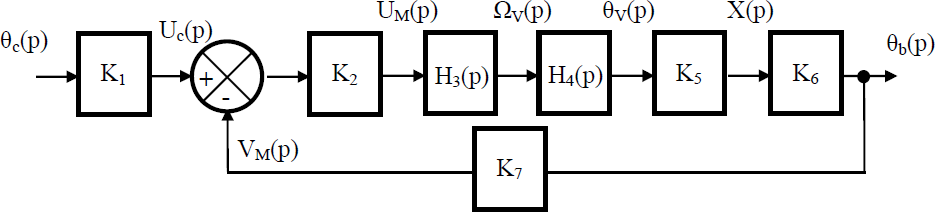
\includegraphics[width=.9\textwidth]{png/fig_3}
\end{center}

Avec $K_1$, $K_2$, $K_5$, $K_6$ et $K_7$ : constantes, $\theta_c(p)$ : angle de consigne, $U_c(p)$ : tension de consigne, $U_M(p)$, tension moteur, $\Omega_V(p)$ : vitesse angulaire de la vis, $\theta_V(p)$ : angle de la vis, $X(p)$ : déplacement de l'écrou, $\dot{\theta_b(p)}$ : position angulaire du bras, $V_M(p)$ : tension mesurée image de $\theta_b(p)$.

\subparagraph{}
\textit{Déterminer le lien entre $K_1$ et $K_7$ pour que $\theta_b(p)$ soit asservi sur $\theta_c(p)$.}

La fonction de transfert $H_3(p)$ est réalisée par un moteur, dont les équations de comportement sont :
$$
u_M(t)=e(t)+R\cdot i(t) \quad e(t)=k_e\omega_v(t) \quad J\cdot \dfrac{d\omega_v(t)}{dt}=C_M(t) \quad C_M(t)=k_M i(t)
$$

Avec $u_M(t)$ : tension aux bornes du moteur (en V), $e(t)$ : force contre-électromotrice (en V), $i(t)$ intensité (en A), $\omega_V(t)$ : vitesse de rotation de la vis en sortie de moteur (en rad/s), $C_M(t)$ ; couple moteur (en N.m) (un couple est une action mécanique qui tend à faire tourner). $J$ inertie équivalente en rotation de l'arbre moteur (en $kg\cdot m^2$), $R$ résistance du moteur (en $\Omega$), $k_e$ constante de force contre-électrmotrice ($V\cdot rad^{-1}\cdot s$), $k_m$ : constante de couple ($N\cdot m\cdot A^{-1}$).

\subparagraph{}
\textit{Déterminer la fonction de transfert $H_3(p)=\dfrac{\Omega_V(p)}{U_M(p)}$. Montrer que $H_3(p)$ peut se mettre sous la forme canonique d'un système du premier ordre où les valeurs $K_3$ et $T_3$ seront à déterminer.}

\subparagraph{}
\textit{Déterminer $\omega_v(t)$ lorsque $u_M(t)$ est un échelon de tension d'amplitude $U_0$. Préciser la valeur de $\omega_v(t)$ à l'origine, la pente de la tangente à l'origine de $\omega_V(t)$ et la valeur finale atteinte par $\omega_V(t)$ lorsque $t$ tend vers l'infini.}

\subparagraph{}
\textit{Déterminer la fonction de transfert $H_4(p)$. }

\subparagraph{}
\textit{Déterminer la fonction de transfert $H(p)=\dfrac{\theta_b(p)}{\theta_c(p)}$. Montrer que cette fonction peut se mettre sous la forme d'un système du second ordre ou les valeurs de $K$, $z$ et $\omega_0$ seront à déterminer.}

La réponse indicielle de $H(p)$ à un échelon unitaire est donnée sur la figure suivante :

\begin{center}
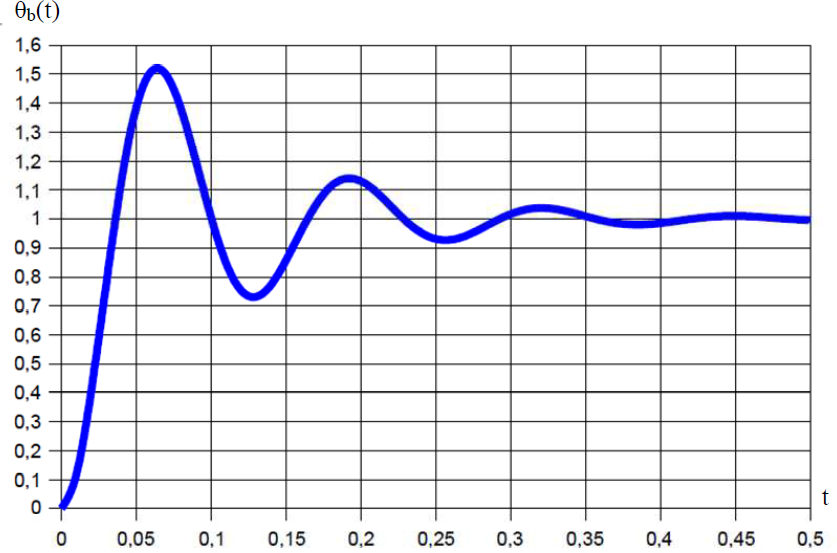
\includegraphics[width=.9\textwidth]{png/fig_4}
\end{center}

\subparagraph{}
\textit{Déterminer, en expliquant la méthode, les valeurs numériques de $K$, $z$ et $\omega_0$.}

\subparagraph{}
\textit{Déterminer, en expliquant la démarche utilisée, le temps de réponse à 5\%. Conclure quant à la capacité du préhenseur à vérifier (ou non) le critère de rapidité de FS1.}

\end{document}
